\section{RF codebook}
\label{sec:intro}


\subsection{Optimizing hyperparameters}
We conducted experiments in a procedure similar to Section2 to find the optimal parameters for the Random Forest vocabulary. The results are shown in \cref{subsec:Q3-app1}. When $N$ (number of trees) = 8, $D$ (depth of trees) = 6, $\rho$ (number of attempts to split per node) = 10, we achieved sufficiently good performance with test accuracy of 60.67\% and the vocabulary size = 256.

\subsection{Comparison with Q2's result}



\begin{figure}[htbp]
	\centering
	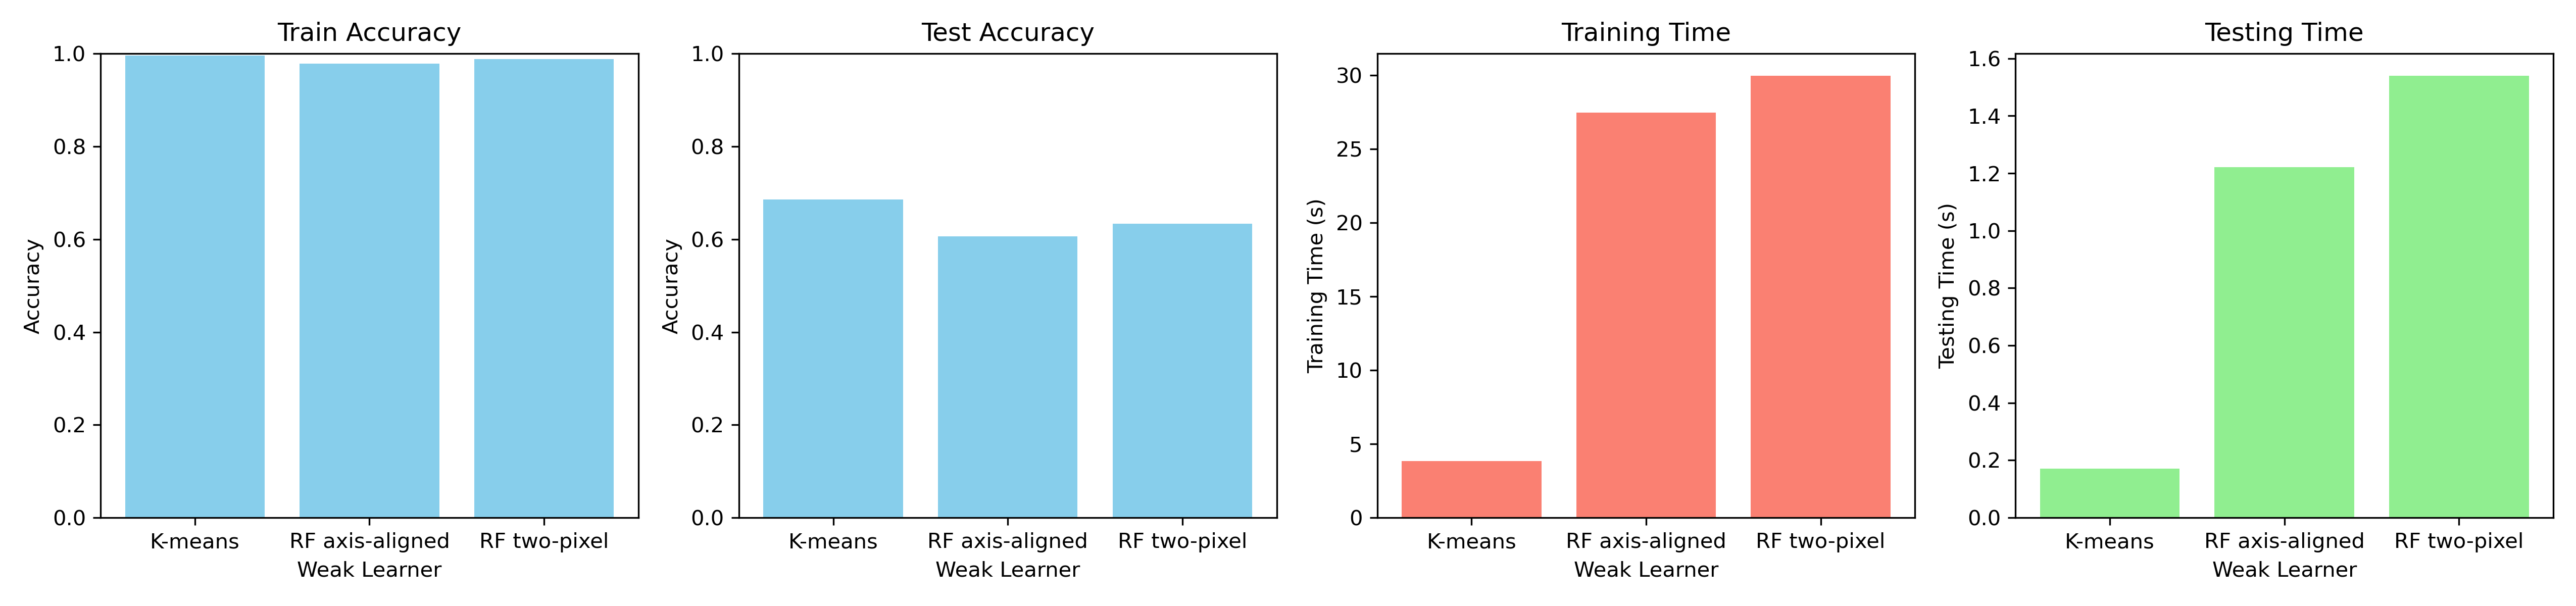
\includegraphics[width=0.8\linewidth]{image/q3-fig4.png}
	\caption{Comparison between different vocabulary method}
	\label{fig:q3-fig4}
\end{figure}